% Hier steht der Rezepttitel
\section{Oma's K\"{o}nigsberger Meatballs}
% Untertitel
\begin{centering}
% Danach die Zutaten in Tabellenform
% Wie viele werden satt?
Serves 10
%\textbf{Zutaten:}
\begin{table}[H]
\centering
% eine Tabelle mit insgesamt 4 Spalten, falls mehr Zutaten benoetigt werden
% links: Menge, rechts: Zutat
\begin{tabular*}{1\textwidth}{rlrl}
%& && \\
35\,oz & ground meat & & lemon juice \\
1$\nicefrac{1}{2}$ & bread rolls & 14.1\,oz / 1$\nicefrac{1}{2}$ cups & sour cream \\
14.1\,oz / 1$\nicefrac{1}{2}$ cups & cr\`{e}me fra\^{i}che &3.5-5\,oz / $\nicefrac{3}{4}$ cup & capers \\
&milk to soak &2x &white gravy powder\\
2-3 & onions & &butter\\
2 & eggs & 35\,oz / 1\,$\ell$ & vegetable broth\\
\end{tabular*}
\end{table}
\end{centering}
%Zubereitung:
\begin{Notes}
\item The night before, soak the bread rolls in milk, thoroughly squeeze out the milk.
\item Cut onions into dices and saut\'{e} onions until transparent, then add the minced meat. Combine and blend with pepper, salt, 2 eggs and bread rolls. 
\item Form meatballs and let steep in vegetable broth for 20\,min.
\item Remove meatballs and stir the white gravy powder into the broth. Add sour cream and cr\`{e}me fra\^{i}che. Together with meatballs and capers once more bring to a boil.
\end{Notes}
\vfill
\begin{figure}[H]
  \centering
  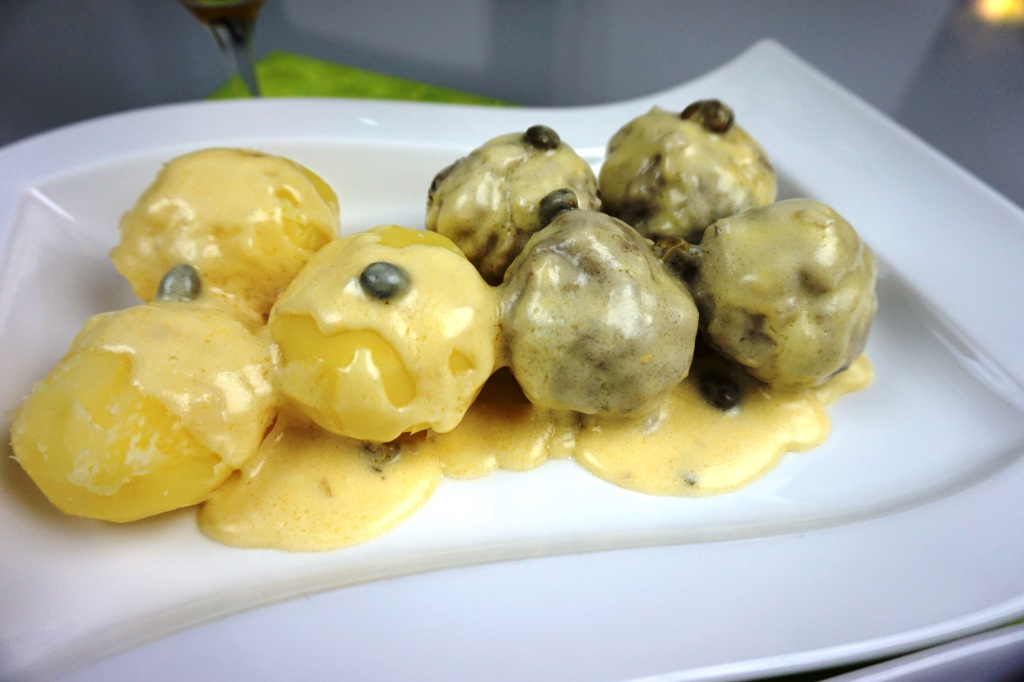
\includegraphics[width=0.75\textwidth]{klopse.JPG}
\end{figure}
\newpage
% Hier steht der Rezepttitel
\section*{Omas K\"{o}nigsberger Klopse}
% Untertitel
\begin{centering}
% Danach die Zutaten in Tabellenform
% Wie viele werden satt?
F\"{u}r 10 Hungrige
%\textbf{Zutaten:}
\begin{table}[H]
\centering
% eine Tabelle mit insgesamt 4 Spalten, falls mehr Zutaten benoetigt werden
% links: Menge, rechts: Zutat
\begin{tabular*}{1\textwidth}{rlrl}
%& && \\
1\,kg & Hackflesich &&Zitronensaft \\
1\nicefrac{1}{2} & Br\"{o}tchen & 2 Becher & Saure Sahne\\
2 Becher & Cr\`{e}me fra\^{i}che &100-150\,g&Kapern\\
&Milch zum Einweichen &2x &helle So{\ss}e (Fertigprodukt)\\
2-3 & Zwiebeln & &Butter\\
2 & Eier & 1\,$\ell$ & Gem\"{u}sebr\"{u}he\\
\end{tabular*}
\end{table}
\end{centering}
%Zubereitung:
\begin{Notes}
\item Am Vorabend Br\"{o}tchen in Milch einweichen, kr\"{a}ftig ausdr\"{u}cken.
\item Zwiebeln w\"{u}rfeln und glasig anbraten, Hackfleisch dazugeben. Mit
Pfeffer, Salz, 2 Eiern, und Br\"{o}tchen durchmengen.
\item Klopse aus der Masse formen und in Gem\"{u}sebr\"{u}he 20\,min ziehen
lassen.
\item Klopse entfernen und die helle So{\ss}e in der Br\"{u}he anr\"{u}hren.
Saure Sahne und Cr\`{e}me fra\^{i}che dazugeben und mit den Klopsen,
zusammen mit den Kapern, aufkochen.
\end{Notes}
\vfill
\begin{figure}[H]
  \centering
  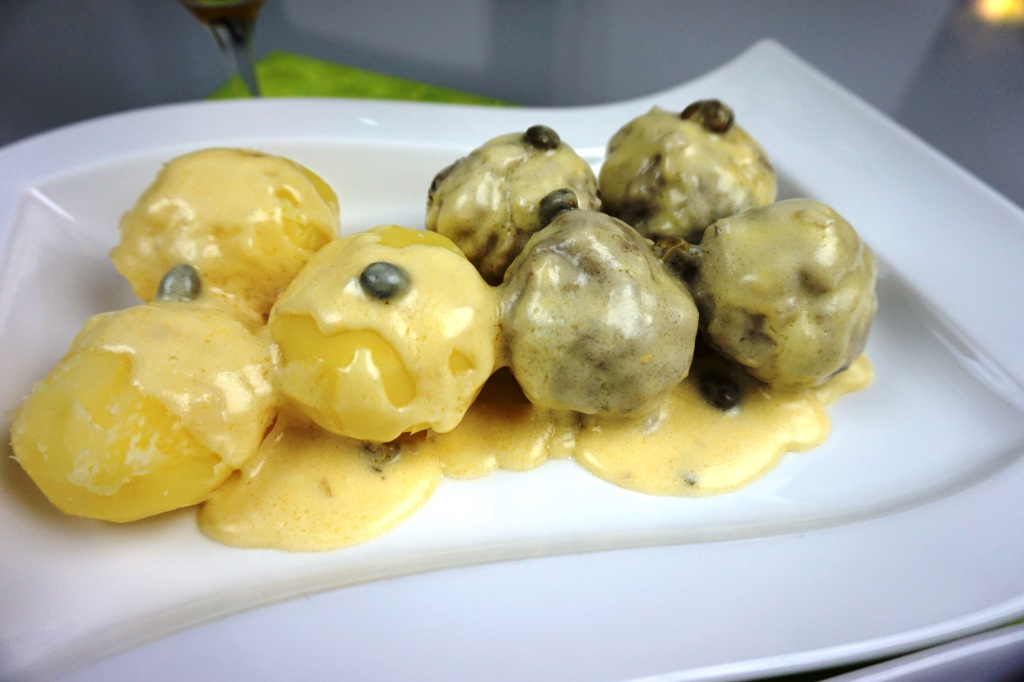
\includegraphics[width=0.75\textwidth]{klopse.JPG}
\end{figure}
\newpage
